\documentclass[11pt,a4paper]{article}

\usepackage[UTF8]{ctex}
\usepackage{amsmath,amssymb,amsthm}
\usepackage{algorithm}
\usepackage{algorithmic}
\usepackage{booktabs}
\usepackage{graphicx}
\usepackage{hyperref}
\usepackage{geometry}
\usepackage{xcolor}

\geometry{margin=1in}

\hypersetup{
  colorlinks=true,
  linkcolor=blue,
  citecolor=blue,
  urlcolor=blue
}

\newtheorem{theorem}{Theorem}
\newtheorem{lemma}{Lemma}
\newtheorem{definition}{Definition}

\title{Paper Review Title}
\author{TODO: Your Name}
\date{\today}

\begin{document}

\maketitle

\begin{abstract}
本文 review 的论文是：\textbf{TODO: paper title}。
本文将依次介绍该论文的研究问题、FLP 之前的相关工作、论文的不可能性证明过程、初始失效进程情形，以及 FLP 之后相关研究如何回应这一理论边界。
\end{abstract}

\tableofcontents

\section{Introduction}

TODO: 介绍被 review 的论文、核心问题、为什么值得研究，以及本文 review 的组织结构。

\section{Problem and Motivation}

TODO: 严格定义论文解决的问题，解释输入、输出、约束、目标函数或评价标准。

TODO: 解释该问题为什么重要，包括理论意义、实际应用或对后续研究的影响。

\section{Related Work Before FLP}

FLP 论文讨论的是异步消息传递系统中的共识不可能性。这个问题并不是孤立出现的；在 FLP 之前，分布式系统、容错计算和分布式数据库领域已经围绕 agreement、commit 和 fault tolerance 形成了多条研究脉络。FLP 的贡献可以放在这些工作之间理解：一方面，它继承了早期 agreement 问题对一致性的关注；另一方面，它把模型收窄到可靠消息、crash failure 和完全异步执行，从而揭示了一个不同于 Byzantine fault 的困难来源。

早期最重要的一条相关研究是 Byzantine agreement。Pease、Shostak 和 Lamport 研究了存在故障处理器时，非故障处理器如何对信息形成一致认识 \cite{pease1980reaching}。他们使用 interactive consistency 的形式化表述，要求所有非故障处理器最终得到相同的信息向量，并且向量中对应非故障处理器的值必须是该处理器真实持有的值。该工作说明，在故障处理器可能向不同接收者发送不同信息时，agreement 问题不能依靠简单多数投票解决，而需要足够的冗余。Lamport、Shostak 和 Pease 随后用 Byzantine Generals problem 将这一类问题表述为经典模型 \cite{lamport1982byzantine}。这些工作关注的是任意或恶意故障，而 FLP 关注的是更弱的 crash failure；这种对比使 FLP 的结论更突出：即使故障进程不会撒谎、不会伪造消息，只是静默停止，完全异步模型仍然会带来根本困难。

另一条与 FLP 动机直接相关的研究线来自分布式数据库中的事务提交。事务提交要求多个数据管理进程一致地决定 commit 或 abort；如果不同副本作出不同决定，数据库状态就会分裂。Dolev 和 Strong 研究了 distributed commit with bounded waiting，试图避免 commit 协议中某些参与者无限等待的问题 \cite{dolev1982distributed}。Skeen 的 nonblocking commit protocols 和 decentralized termination protocol 进一步分析了提交协议中哪些状态会导致 blocking，以及在站点故障后如何推动事务进入最终决定 \cite{skeen1981nonblocking,skeen1982decentralized}。Skeen 和 Stonebraker 则从 crash recovery 角度形式化分布式系统在故障和恢复后的状态一致性问题 \cite{skeen1983formal}。这些工作表明，FLP 论文中的 transaction commit 例子不是附带说明，而是当时分布式数据库系统面临的实际问题：系统既要保持一致性，又希望在故障出现后不无限等待。

\section{证明过程}

该论文的核心不是给出一个新的共识协议，而是证明在特定模型下这样的协议不可能存在。为了使证明结构与原论文一致，本节先给出必要的状态机定义，然后按“引理及其证明”的顺序说明整个不可能性证明。

\subsection{预备定义}

论文把一个共识协议形式化为由若干进程组成的异步状态机系统。每个进程都有输入寄存器、输出寄存器、程序计数器和内部存储。输入寄存器保存该进程的初始输入，输出寄存器的初始值表示尚未决定；当输出寄存器被写成 $0$ 或 $1$ 时，该进程进入决定状态。输出寄存器一旦被写入决定值就不能再改变。

每个进程按照确定性的状态转移函数运行。也就是说，只要给定该进程当前的内部状态和本次收到的消息，它下一步进入什么状态、发送哪些消息，都是确定的。不过，协议的确定性并不意味着系统只有一条执行路径，因为在异步系统中，下一步由哪个进程执行、哪条消息先被投递，仍然可以有不同选择。

整个系统的状态称为一个构型。一个构型包括所有进程的内部状态，以及消息缓冲区中已经发送但尚未投递的消息。初始构型是指所有进程处于初始状态，且消息缓冲区为空的构型。

一次基本执行步骤由某个进程完成。该进程先从消息系统接收一条消息；如果此时没有消息被投递，也可以收到一个空标记。随后，该进程根据当前内部状态和收到的消息进行状态转移，并向其他进程发送有限条消息。由于进程的状态转移函数是确定的，所以一次步骤可以由一个事件表示：

\[
e=(p,m),
\]

其中 $p$ 表示执行步骤的进程，$m$ 表示该进程收到的消息或空标记。从构型 $C$ 应用事件 $e$ 后得到的新构型记为 $e(C)$。一串可以依次应用的事件称为一个调度；从某个构型出发，经过有限调度能够到达的构型称为可达构型。

如果某个构型中已经有进程进入决定状态，并且输出值为 $v$，那么该构型具有决定值 $v$。论文要求部分正确性满足两个条件。第一，任何可达构型都不能同时具有两个不同的决定值；这对应共识的一致性。第二，对于 $0$ 和 $1$，都必须存在某些可达构型以该值作为决定值；这排除了所有进程永远固定决定同一个常数的平凡协议。

论文还定义了执行中的故障。若一个进程在某次无限执行中执行了无限多步，则它是非故障进程；否则它是故障进程。一次执行是容许执行，当且仅当它最多包含一个故障进程，并且所有发送给非故障进程的消息最终都会被接收。一次执行是决定执行，当且仅当至少有一个进程在该执行中进入决定状态。

因此，所谓能够容忍一个故障的完全正确共识协议，是指该协议既满足部分正确性，又保证每个容许执行都是决定执行。该论文的主定理就是证明不存在这样的协议。

在进入引理之前，还需要说明二价构型和单价构型。对于任意构型 $C$，考虑从 $C$ 出发所有可达构型中可能出现的决定值集合。如果这个集合同时包含 $0$ 和 $1$，则称 $C$ 为二价构型。也就是说，从这个构型继续执行，系统未来既可能决定 $0$，也可能决定 $1$。如果从构型 $C$ 出发，所有可能的未来决定值都只能是同一个值，则称 $C$ 为单价构型。若唯一可能的决定值是 $0$，则称为 $0$ 单价构型；若唯一可能的决定值是 $1$，则称为 $1$ 单价构型。

二价和单价描述的不是当前是否已经决定，而是从当前构型继续执行时，未来可能达到的决定值范围。

\subsection{引理一：互不相关调度的交换性}

引理一说明的是状态机执行中的一个基本事实。设从同一个构型 $C$ 出发，两个调度分别到达构型 $C_1$ 和 $C_2$。如果这两个调度中执行步骤的进程集合互不相交，那么这两个调度可以交换先后顺序：先执行第一个调度再执行第二个调度，和先执行第二个调度再执行第一个调度，最终会到达同一个构型。

\paragraph{证明。}

这个结论直接来自状态机模型。两个调度作用在互不相交的进程集合上，因此它们改变的是不同进程的内部状态。由于进程的状态转移是局部的，一个调度不会改变另一个调度所涉及进程的内部状态，所以二者的先后顺序不会影响最终得到的全局构型。后续证明会使用这个交换性来比较不同执行路径。

\begin{figure}[htbp]
  \centering
  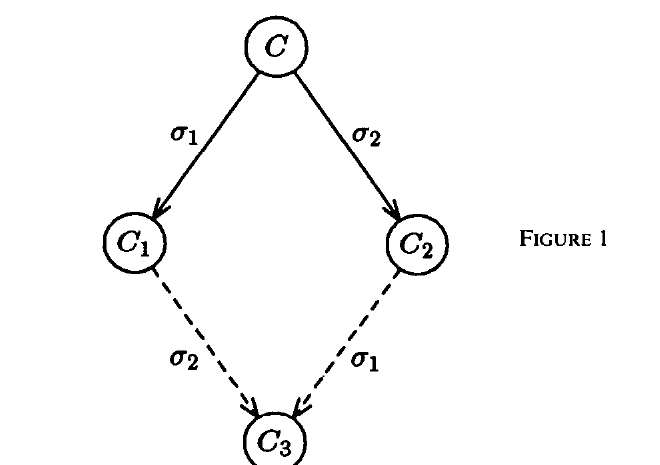
\includegraphics[width=0.52\textwidth]{figures/flp-figure-1.png}
  \caption{原论文图 1：两个互不相关调度的交换性。}
  \label{fig:flp-commutativity}
\end{figure}

\subsection{引理二：存在二价初始构型}

引理二要证明：如果协议能够容忍一个故障并且完全正确，则它必然存在一个二价初始构型。

\paragraph{证明。}

证明采用反证法。假设不存在二价初始构型，那么每个初始构型都是单价构型。由于协议满足部分正确性，$0$ 和 $1$ 都必须在某些可达构型中作为决定值出现，因此初始构型中既必须存在 $0$ 单价构型，也必须存在 $1$ 单价构型。

在论文中，如果两个初始构型只在一个进程的初始输入值上不同，就把它们称为相邻初始构型。任意两个初始构型都可以通过一串相邻初始构型连接起来。因此，在从某个 $0$ 单价初始构型过渡到某个 $1$ 单价初始构型的链条上，一定存在两个相邻初始构型 $C_0$ 和 $C_1$，其中 $C_0$ 是 $0$ 单价，$C_1$ 是 $1$ 单价，且二者只在某个进程 $p$ 的初始输入上不同。

现在考虑从 $C_0$ 出发的一次容许决定执行，并要求进程 $p$ 在该执行中不执行任何步骤。这仍然符合最多一个故障进程的要求。设这次执行对应的调度为 $\sigma$。由于 $C_0$ 和 $C_1$ 的差异只存在于进程 $p$ 的内部初始状态，而 $\sigma$ 中进程 $p$ 不执行步骤，所以同一个调度 $\sigma$ 也可以应用于 $C_1$。在这两次执行中，除进程 $p$ 之外，其他进程看到的状态变化相同，因此最终决定值也必须相同。

如果这个共同决定值是 $1$，则 $C_0$ 不可能是 $0$ 单价；如果这个共同决定值是 $0$，则 $C_1$ 不可能是 $1$ 单价。两种情况都与前面的假设矛盾。因此，协议必然存在一个二价初始构型。

\subsection{引理三：二价构型可以延续}

引理三要证明：从任意二价构型出发，对于任意一个可以应用的事件，都可以找到一种合法的有限调度，使得该事件作为最后一步被执行后，系统仍然到达某个二价构型。

\paragraph{证明。}

设当前构型 $C$ 是二价构型，事件 $e=(p,m)$ 可以应用于 $C$。令集合 $\mathcal{C}$ 表示所有从 $C$ 出发、在没有应用事件 $e$ 的情况下可达的构型。再令集合 $\mathcal{D}$ 表示对 $\mathcal{C}$ 中构型应用事件 $e$ 后得到的构型集合。要证明的是，$\mathcal{D}$ 中至少包含一个二价构型。

证明仍采用反证法。假设 $\mathcal{D}$ 中没有二价构型，那么 $\mathcal{D}$ 中每个构型都是单价构型。由于 $C$ 是二价构型，从 $C$ 出发既能到达导致决定 $0$ 的构型，也能到达导致决定 $1$ 的构型。由此可以推出，$\mathcal{D}$ 中既包含 $0$ 单价构型，也包含 $1$ 单价构型。

接着考虑集合 $\mathcal{C}$ 中两个相邻构型 $C_0$ 和 $C_1$。这里的相邻构型和引理二中的相邻初始构型不同：这里的相邻是指一个构型可以通过一个事件到达另一个构型。由于 $\mathcal{D}$ 中既有 $0$ 单价构型也有 $1$ 单价构型，沿着从 $C$ 出发的一条有限调度路径，应用事件 $e$ 后得到的单价类型必然在某一步发生变化。因此，可以找到这样的相邻构型 $C_0$ 和 $C_1$，它们只相差一个事件 $e'=(p',m')$，并且

\[
C_1=e'(C_0).
\]

对它们分别应用事件 $e$，得到

\[
D_0=e(C_0), \qquad D_1=e(C_1),
\]

其中 $D_0$ 是 $0$ 单价构型，$D_1$ 是 $1$ 单价构型。也就是说，在应用同一个事件 $e$ 后，这两个相邻构型分别变成了不同的单价构型。下面分两种情况讨论。

第一种情况是 $p'\neq p$。此时事件 $e'$ 和事件 $e$ 发生在不同进程上。根据引理一，这两个事件可以交换顺序。因此，从 $D_0$ 再应用 $e'$ 可以到达 $D_1$，如图 \ref{fig:flp-case-one} 所示。但是 $D_0$ 已经是 $0$ 单价构型，它的后继构型不可能是 $1$ 单价构型，否则就说明从 $D_0$ 出发仍可能决定 $1$。这产生矛盾。

\begin{figure}[htbp]
  \centering
  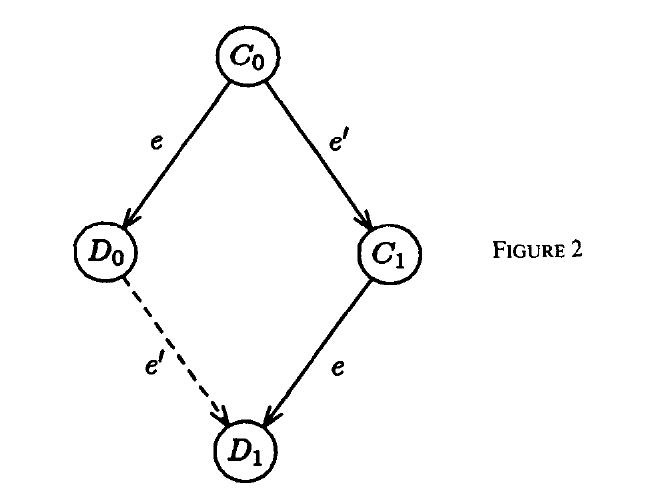
\includegraphics[width=0.52\textwidth]{figures/flp-figure-2.png}
  \caption{原论文图 2：引理三中 $p'\neq p$ 时的交换关系。}
  \label{fig:flp-case-one}
\end{figure}

第二种情况是 $p'=p$。此时 $e'$ 和 $e$ 都发生在同一个进程 $p$ 上，因此不能直接交换 $e'$ 和 $e$ 的先后顺序。论文转而选择一段不涉及进程 $p$ 的调度。具体地说，从 $C_0$ 出发，令进程 $p$ 不执行任何步骤。由于协议被假设为能够容忍一个故障并且完全正确，这仍然是一种允许的情形，所以存在一段有限调度使系统产生决定。设这段调度为 $\sigma$，并记

\[
A=\sigma(C_0).
\]

这里 $\sigma$ 中没有进程 $p$ 的步骤，而 $e'$ 和 $e$ 都是进程 $p$ 的事件。因此，可以交换的不是 $e'$ 与 $e$，而是整段调度 $\sigma$ 与进程 $p$ 的事件序列。

先看从 $A$ 出发执行事件 $e$。一方面，这条路径可以写成

\[
C_0 \xrightarrow{\sigma} A \xrightarrow{e} e(A).
\]

另一方面，由于 $\sigma$ 不涉及进程 $p$，它可以越过事件 $e$，所以这条路径等价于

\[
C_0 \xrightarrow{e} D_0 \xrightarrow{\sigma} \sigma(D_0).
\]

因此，$e(A)$ 与 $\sigma(D_0)$ 是同一个结果。又因为 $D_0$ 是 $0$ 单价构型，而单价构型的后继仍然只能保持同一个决定值，所以从 $A$ 出发至少可以到达一个 $0$ 单价构型。

再看从 $A$ 出发先执行 $e'$、再执行 $e$。这条路径可以写成

\[
C_0 \xrightarrow{\sigma} A \xrightarrow{e'} e'(A) \xrightarrow{e} e(e'(A)).
\]

同样，由于 $\sigma$ 不涉及进程 $p$，而 $e'$ 和 $e$ 都只涉及进程 $p$，整段 $\sigma$ 可以越过这两个事件，放到它们之后执行。于是上面的路径等价于

\[
C_0 \xrightarrow{e'} C_1 \xrightarrow{e} D_1 \xrightarrow{\sigma} \sigma(D_1).
\]

因此，$e(e'(A))$ 与 $\sigma(D_1)$ 是同一个结果。又因为 $D_1$ 是 $1$ 单价构型，所以从 $A$ 出发也可以到达一个 $1$ 单价构型。

这样，从同一个构型 $A$ 出发，既存在通向 $0$ 单价构型的后继路径，也存在通向 $1$ 单价构型的后继路径。因此，按照二价构型的定义，$A$ 应当是二价构型。

\begin{figure}[htbp]
  \centering
  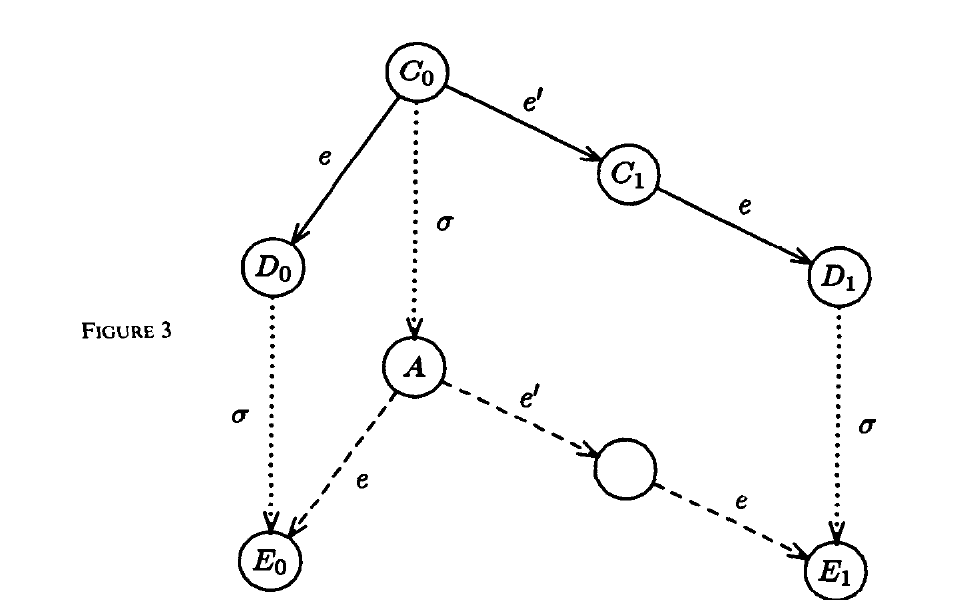
\includegraphics[width=0.78\textwidth]{figures/flp-figure-3.png}
  \caption{原论文图 3：引理三中 $p'=p$ 时，调度 $\sigma$ 与进程 $p$ 的事件序列之间的交换关系。}
  \label{fig:flp-case-two}
\end{figure}

但是，$\sigma$ 是一段决定执行，所以到达的构型 $A$ 已经具有某个决定值。根据一致性要求，一个已经具有决定值的可达构型不可能仍然同时通向两个不同决定值。因此 $A$ 必须是单价构型。这与刚刚推出的 $A$ 为二价构型矛盾。

两种情况都导致矛盾，所以反证假设不成立。因此，集合 $\mathcal{D}$ 中必然存在二价构型。这说明，从一个二价构型出发，即使指定某个事件最终要发生，也总可以先安排一段有限调度，使该事件发生后系统仍保持二价。

\subsection{主定理：不存在能容忍一个故障的完全正确共识协议}

主定理要证明：在完全异步消息传递系统中，只要允许一个进程崩溃，就不存在一个确定性共识协议能够保证所有容许执行都产生决定。

\paragraph{证明。}

证明采用反证法。假设存在这样一个协议，它能够容忍一个故障并且完全正确。根据引理二，存在一个二价初始构型。执行从这个构型开始。

接下来利用引理三构造一条无限执行。论文维护一个进程队列，并将消息缓冲区中的消息按照发送时间排序。每一阶段都选择队首进程 $p$，并令 $m$ 为当前发给 $p$ 的最早消息；如果没有这样的消息，则令 $m$ 为空标记。于是得到事件 $e=(p,m)$。

由于当前阶段开始时的构型保持为二价构型，根据引理三，存在一段有限调度，使得事件 $e$ 作为最后一步被执行，并且执行结束后系统仍然到达某个二价构型。论文把这段有限调度作为当前阶段。随后将进程 $p$ 移到队列末尾，进入下一阶段。

这个过程可以无限重复，因为每一阶段结束时仍然得到二价构型。按照队列轮转方式，每个进程都会不断获得执行机会；按照选择最早消息的方式，发给非故障进程的消息最终都会被接收。因此，构造出的无限执行是容许执行。

另一方面，这条执行中每个阶段结束时系统都处于二价构型。如果某个进程已经进入决定状态，那么当前构型就已经具有某个决定值，并且由于协议满足一致性，它不可能仍然是二价构型。因此，在这条无限执行中没有进程进入决定状态。

于是得到一条容许执行，但它不是决定执行。这与完全正确性的要求矛盾。由此可知，假设中的确定性共识协议不存在。主定理得证。

\section{初始失效进程情形}

在完成主定理证明之后，原论文还讨论了一个不同的故障情形：进程可能在协议开始前就已经失效，但协议执行过程中不会再有新的进程死亡。这个部分并不是主定理证明的一环，而是用来说明不可能性结果的适用边界。

主定理考虑的是执行过程中可能发生崩溃的完全异步共识。在这种模型下，某个进程长时间没有行动，其他进程无法区分它是已经崩溃，还是只是运行很慢。正是这种不可区分性，使协议无法同时保证一致性和终止性。初始失效进程情形则改变了故障假设：哪些进程已经失效在执行开始时就固定下来，之后存活进程不再发生新的崩溃。

在这一较弱的故障模型下，原论文给出一个正向结果：如果初始时存活的进程占严格多数，并且执行过程中没有进程继续死亡，那么存在一个部分正确的共识协议，使所有非故障进程最终都能作出决定。这个结论说明，FLP 不可能性并不是说只要系统中存在不可用进程，共识就一定无法解决；它针对的是更困难的动态崩溃情形。

原论文中的协议大致分为两个阶段。第一阶段，每个存活进程广播自己的进程编号，并等待收到足够多其他进程的消息。根据“哪个进程收到了哪个进程的消息”，系统可以形成一个有向图。图中的节点对应进程，如果进程 $j$ 收到了进程 $i$ 的消息，就在图中加入从 $i$ 到 $j$ 的边。

第二阶段，进程继续交换自己已经知道的图信息和初始值信息，从而逐步获得关于图的传递可达关系。每个完成协议的进程最终都能识别出同一个初始团。这里的初始团可以理解为一个没有外部入边的共同进程集合。由于初始存活进程占严格多数，论文证明这样的初始团是唯一的，并且每个完成第二阶段的进程都能知道这个集合及其成员的初始值。

最后，所有进程根据这个共同初始团中进程的初始值，使用同一个预先约定的规则作出决定。由于完成协议的进程识别出的初始团相同，且它们使用的决定规则也相同，所以它们会得到相同的决定值。这保证了一致性；同时，在该模型假设下，非故障进程能够完成两个阶段，因此也能最终决定。

这一部分和主定理的关系可以概括为对照关系。主定理证明的是：在完全异步系统中，如果允许进程在执行过程中崩溃，则不存在确定性协议能够保证所有容许执行都终止。初始失效进程部分则说明：如果把故障限制为协议开始前已经发生，并要求执行过程中没有新的崩溃，那么在多数进程存活的条件下，共识仍然可以解决。因此，它帮助界定了 FLP 结果的真正含义：困难不只是“有进程不可用”，而是“进程可能在异步执行过程中停止，且其他进程无法判断它是慢还是死”。

\section{FLP 之后的相关工作}

FLP 之后，一类直接回应是不再坚持确定性终止，而是引入随机化。Ben-Or 提出了完全异步系统中的随机化一致性协议 \cite{benor1983advantage}。该工作明确以 FLP 的不可能性为背景：既然确定性协议无法在完全异步系统中保证终止，那么可以让进程使用随机选择，并将终止保证改为概率意义上的终止。Ben-Or 的协议并不推翻 FLP，而是改变了问题要求。Bracha 和 Toueg 对弹性共识协议的研究也属于这一方向 \cite{bracha1983resilient}。这类工作说明，FLP 的影响不是让共识研究停止，而是迫使后续协议明确说明自己在哪些要求上不同于 FLP 的原始模型。

另一类回应是弱化完全异步模型，加入更符合实际系统的时序假设。Dwork、Lynch 和 Stockmeyer 提出了部分同步模型 \cite{dwork1988consensus}。完全同步模型假设消息延迟和处理速度有已知上界；完全异步模型则完全没有这样的上界。部分同步位于两者之间：系统可能存在某些上界，但这些上界可能未知，或者只在某个全局稳定时间之后才成立。这个模型解释了为什么现实系统常常可以使用超时、领导者和重试机制：这些机制并不是在纯粹异步模型中无条件可靠，而是依赖某种最终稳定的时间假设。

故障检测器理论则从另一个角度回应 FLP。FLP 的核心困难之一是进程无法判断另一个进程是已经崩溃，还是只是运行很慢。Chandra 和 Toueg 引入不可靠故障检测器，用完备性和准确性刻画故障检测器可能提供的信息，并证明即使故障检测器可能犯错，某些类型的检测器仍足以帮助异步崩溃故障系统解决共识问题 \cite{chandra1996unreliable}。Chandra、Hadzilacos 和 Toueg 进一步研究解决共识所需的最弱故障检测器 \cite{chandra1996weakest}。这条研究线把 FLP 的直觉转化为更精确的问题：完全异步系统缺少关于故障的信息；若要重新获得共识可解性，至少需要补充多少信息？

在系统实现层面，FLP 之后的研究将共识与复制服务、日志复制和容错系统构建联系起来。Schneider 的状态机方法将容错服务建模为多个确定性状态机副本按相同顺序执行相同命令 \cite{schneider1990state}。这一路线把共识变成实现复制状态机的关键子问题：只要所有副本对操作顺序达成一致，它们就能保持一致状态。Lamport 的 Paxos 系列工作进一步给出了崩溃故障场景下影响深远的共识协议 \cite{lamport1998part,lamport2001paxos}。Paxos 使用轮次编号、法定集合和多数派交集保证安全性，并在实际系统中配合领导者、重试和超时机制获得进展。Paxos 并不违反 FLP；它的活性依赖额外的进展假设，而其价值在于把这些假设组织成可实现的协议框架。

后续系统工作还将共识思想推广到更强故障模型或更易实现的协议结构。Castro 和 Liskov 的 PBFT 将状态机复制推向实用拜占庭容错，在 $3f+1$ 个副本中容忍 $f$ 个拜占庭故障副本 \cite{castro1999practical}。Ongaro 和 Ousterhout 的 Raft 则针对 Paxos 难以理解和实现的问题，将复制日志共识分解为领导者选举、日志复制、安全性和成员变更等部分 \cite{ongaro2014search}。这些工作共同说明，FLP 不可能性结果并没有否定现实系统中的共识服务；相反，它促使后续研究在提出协议时更明确地区分安全性、活性以及协议所依赖的时序、故障检测、多数派或随机化假设。

综上，FLP 之后的相关研究主要沿三类方向展开。第一，随机化、部分同步和故障检测器等工作直接回应 FLP，展示如何通过改变模型假设或终止要求恢复共识可解性。第二，状态机复制、Paxos、PBFT 和 Raft 等系统化工作说明，共识最终成为构建容错服务的核心工具。第三，这些后续工作共同表明，实际系统必须清楚说明自己依赖了哪些超出完全异步模型的条件。

\section{Conclusion}

TODO: 总结这篇论文的贡献、技术洞见和这篇 review 的核心判断。


\bibliographystyle{plain}
\bibliography{references}

\end{document}
